\documentclass[11pt,a4paper]{article}
\usepackage[utf8]{inputenc}
\usepackage[margin=2.3cm]{geometry}
\usepackage{graphicx}
\usepackage{booktabs}
\usepackage{tabularx}
\usepackage{amsmath,amssymb}
\usepackage{xcolor}
\usepackage{enumitem}
\usepackage{fancyhdr}
\usepackage{url}

\definecolor{navy}{HTML}{14213A}
\graphicspath{{../png/}}
\setlist{itemsep=2pt,topsep=4pt}
\newcommand{\cat}{\,\|\,}
\newcommand{\GF}{\mathrm{GF}(2^{128})}

\pagestyle{fancy}
\fancyhf{}
\fancyhead[L]{\small BITS F463: Cryptography --- Streaming AEAD over AES-GCM}
\fancyhead[R]{\small Group 4}
\fancyfoot[C]{\thepage}

\begin{document}

\begin{titlepage}
\centering
\vspace*{2.5cm}
{\large\scshape BITS F463: Cryptography\par}
\vspace{1.2cm}
{\Huge\bfseries\color{navy} Streaming AEAD over AES-GCM\par}
\vspace{0.4cm}
{\Large Encrypting Files of Any Size in Constant Memory\par}
\vspace{1cm}
\rule{0.7\textwidth}{0.4pt}\par
\vspace{1cm}
{\Large\bfseries Final Project Report\par}
\vspace{2cm}
{\large\bfseries Group 4\par}
\vspace{0.4cm}
\begin{tabular}{ll}
Haider Abuzer Salik & 2024A7PS0691G\\
Aadi Kawalay & 2024A7PS0504G\\
Bhagyesh Kamal & 2024ADPS0863G\\
Mohammad Zaid Agha & 2024ADPS0840G
\end{tabular}
\vfill
Project repository:\\
\url{https://github.com/SupercalifragilisticexpialidociousPoppy/streaming-aes}
\end{titlepage}

\begin{abstract}
AES-GCM authenticates a message as one unit, so a safe one-shot decryptor must hold the whole message in memory, and NIST limits a single GCM message to about 64\,GiB. We designed and implemented a chunked file format over AES-256-GCM that encrypts files of any size in constant memory. Each 1\,MiB chunk is a separate GCM call whose nonce encodes the chunk's position and whether it is the last chunk, under a key derived for each file from the master key, a random salt and the whole header (HKDF-SHA256). We also implemented GCM itself, validated against all 47,250 NIST test vectors. Four attacks that move valid chunks (truncation, reordering, replay, splicing) succeed against a naive chunked design and fail against ours; a fifth, IV reuse, breaks GCM itself, and we show how our design makes it practically impossible. The engine uses about 3\,MiB of memory for any file size, against 512\,MiB for one-shot GCM on a 256\,MiB file.
\end{abstract}

\setcounter{tocdepth}{1}
\tableofcontents
\newpage

%=====================================================================
\section{Introduction}

Authenticated encryption keeps data secret and detects any change to it. AES-GCM is the most widely used authenticated encryption scheme: counter mode provides secrecy, and a polynomial hash over $\GF$ provides a 16-byte authentication tag~\cite{mv-spec,sp80038d}. GCM processes one whole message at a time, which causes two problems for large files.

\paragraph{Memory.} A decryptor must not release plaintext before the tag verifies (\emph{verify-then-release}), and the tag covers the whole message. A simple safe implementation therefore buffers the whole file: encrypting a 256\,MiB file with a one-shot API used 512\,MiB of memory in our measurements. Python's \texttt{AESGCM} refuses inputs over $2^{31}-1$ bytes altogether.

\paragraph{A hard limit.} GCM numbers its 16-byte blocks with a 32-bit counter. One value is reserved for the tag and the counter may not wrap, so a message holds at most $2^{32}-2$ blocks, that is $(2^{32}-2)\times 128 = 2^{39}-256$ bits, about 64\,GiB~\cite{sp80038d}.

Splitting a file into chunks and encrypting each separately solves both problems, but done naively it is unsafe: every chunk still passes its own tag check while an attacker deletes, reorders, repeats or swaps chunks, and a careless nonce scheme can repeat an IV under the same key, which breaks GCM completely~\cite{joux}.

\paragraph{Objectives.}
\begin{enumerate}
\item Implement GCM from its definition and validate it against NIST's test vectors.
\item Design a chunked file format that protects the file as a whole, not just each chunk.
\item Build a streaming engine with constant memory and all-or-nothing output.
\item Implement a naive chunked design and demonstrate the attacks it allows, against both designs.
\item Measure throughput, memory and the cost of our own GCM.
\end{enumerate}

%=====================================================================
\section{Literature survey}

\subsection{AES-GCM}
McGrew and Viega introduced the Galois/Counter Mode~\cite{mv-spec,mv-sec}, standardised by NIST in SP 800-38D~\cite{sp80038d}. With AES~\cite{fips197} written $E_K$, a 96-bit IV gives the pre-counter block $J_0 = IV \cat 0^{31} \cat 1$, and counter blocks $J_i = \mathrm{inc}_{32}(J_{i-1})$ increment the last 32 bits. Encryption is counter mode, $C_i = P_i \oplus E_K(J_i)$. The hash subkey is $H = E_K(0^{128})$, and GHASH processes the blocks $B_1,\dots,B_m$ of the associated data $A$, the ciphertext $C$ (each zero-padded) and a block holding both lengths:
\[
X_0 = 0,\quad X_i = (X_{i-1} \oplus B_i)\cdot H, \qquad \mathrm{GHASH}_H(A, C) = X_m = \bigoplus_{i=1}^{m} B_i\, H^{m-i+1}.
\]
The tag is $T = \mathrm{GHASH}_H(A,C) \oplus E_K(J_0)$ (Figure~\ref{fig:gcm}). The standard defines GCM only in terms of the block cipher $E_K$ and its counter mode; it never uses ECB mode.

\begin{figure}[ht]
\centering
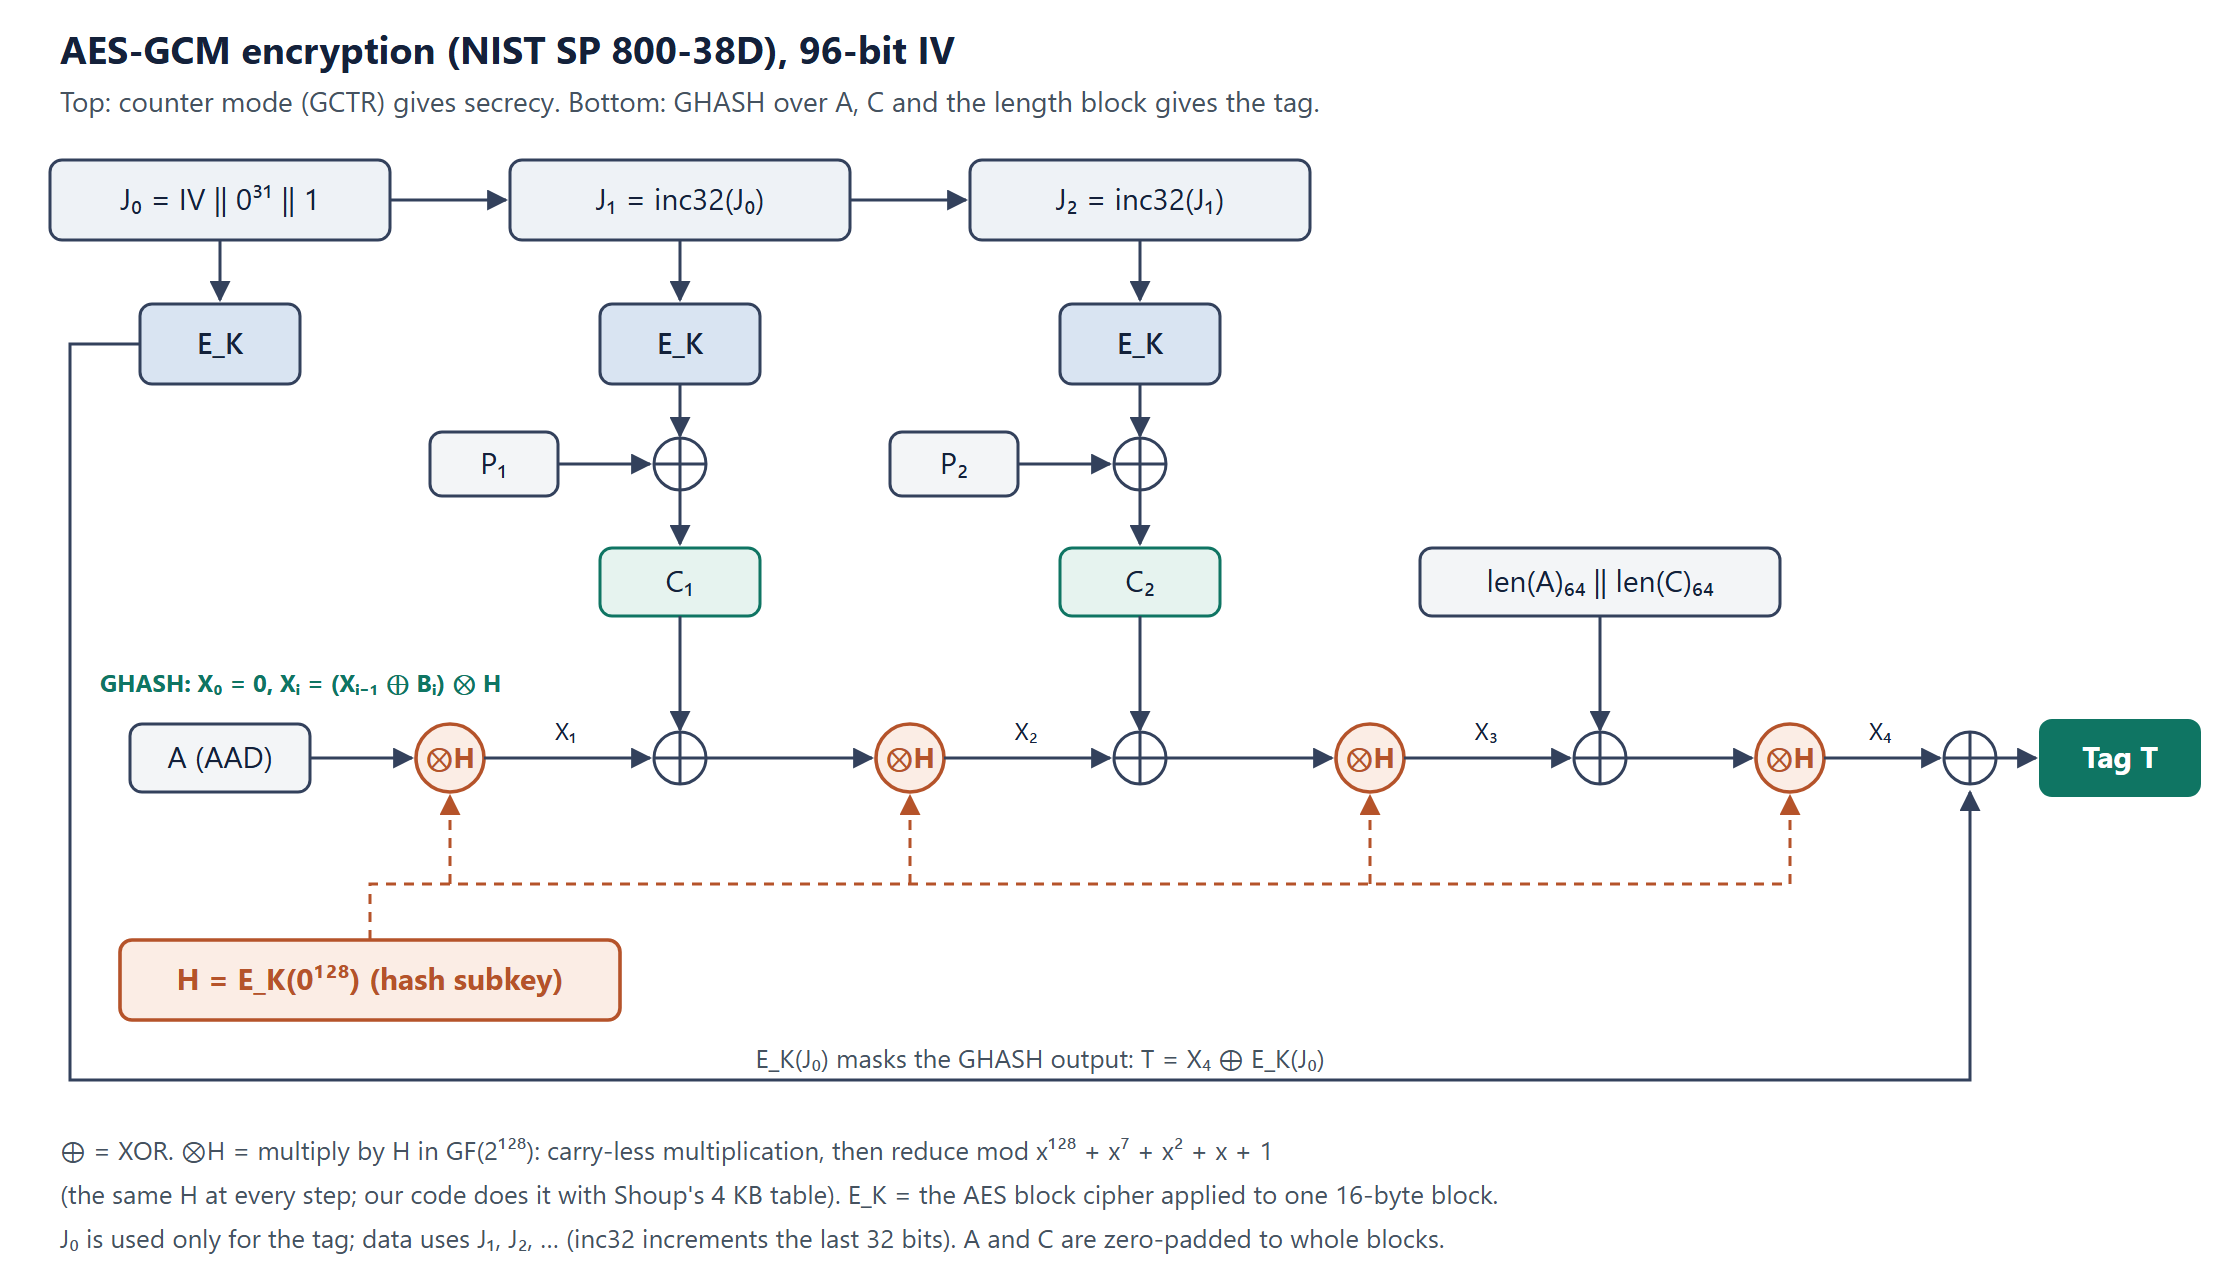
\includegraphics[width=\textwidth]{gcm_diagram.png}
\caption{AES-GCM encryption, drawn from NIST SP 800-38D. $H = E_K(0^{128})$ feeds every multiplication; $\otimes H$ is multiplication in $\GF$.}
\label{fig:gcm}
\end{figure}

\subsection{Arithmetic in $\GF$ and the security of GHASH}
A 128-bit block is a polynomial with binary coefficients; addition is XOR and multiplication is polynomial multiplication modulo the irreducible $x^{128}+x^7+x^2+x+1$. Because a non-zero polynomial of degree $\ell$ has at most $\ell$ roots, a forgery attempt on an $\ell$-block message succeeds with probability about $\ell/2^{128}$, and McGrew and Viega bound the confidentiality advantage by $(\sigma+2q)^2/2^{129}$ for $\sigma$ blocks in $q$ messages~\cite{mv-sec}. Iwata, Ohashi and Minematsu later found and repaired a flaw in this proof for IVs that are not 96 bits~\cite{iom}. Shoup's table method speeds up multiplication by a fixed $H$ using precomputed tables~\cite{shoup}.

\subsection{IV reuse: the forbidden attack}
GCM is not robust to IV reuse. Two messages under the same key and IV share a keystream, so one known plaintext reveals the other; worse, their tags give a polynomial equation in $H$ whose roots reveal $H$, after which tags can be forged for any message~\cite{joux}. Hoang et al.\ study nonce-reuse resistance formally~\cite{hrrv}; GCM does not have it, so a design built on GCM must prevent IV reuse structurally.

\subsection{Online and streaming authenticated encryption}
Hoang, Reyhanitabar, Rogaway and Viz\'ar define the STREAM construction~\cite{hrrv}: a message is split into segments, and each segment is encrypted with a nonce that encodes its index and a flag marking the last segment, so the security of the whole stream reduces to that of the underlying AEAD. Google Tink's streaming AEAD~\cite{tink} uses STREAM over AES-GCM with a per-stream key derived by HKDF, and the \texttt{age} file format~\cite{age} uses it over ChaCha20-Poly1305 with 64\,KiB chunks. The TLS~1.3 record layer~\cite{rfc8446} uses a related idea: a per-record sequence number mixed into the nonce, with an authenticated close message to detect truncation.

\subsection{Key derivation}
HKDF~\cite{rfc5869} derives keys from secret input with HMAC-SHA256 in two steps: \emph{extract} mixes the input key with a salt into a uniform key, and \emph{expand} produces the output key, labelled by an \emph{info} string. Different salts or labels give unrelated keys, and the output reveals nothing about the input key.

\subsection{Conformance testing}
NIST's Cryptographic Algorithm Validation Program publishes known-answer test vectors for GCM encryption and decryption~\cite{cavp}, covering all AES key sizes, several IV and tag lengths, and records that must be rejected.

%=====================================================================
\section{Methodology}

\subsection{Threat model}
The attacker can read and rewrite everything on the wire or on disk: flip bits, drop, reorder, duplicate or substitute chunks, and edit the header, but never sees a key. We aim for confidentiality, integrity of every chunk, integrity of the stream as a whole (order, completeness, origin), and all-or-nothing output. A loop of independent GCM calls provides only the first two.

\subsection{Reference GCM implementation}
We implemented GCM in Python: $\GF$ multiplication, GHASH, the counter blocks, counter mode and the tag. AES itself comes from the \texttt{cryptography} library (OpenSSL). Following SP 800-38D, AES is used only as $E_K$ and as GCM's counter mode, both built on the library's CTR mode: CTR started at block $X$ over 16 zero bytes outputs exactly $E_K(X)$, and counter mode is restarted where GCM's 32-bit counter wraps. No ECB mode is used. Multiplication by $H$ uses Shoup's 4\,KB table of $H$ times every byte value, so each multiplication is 16 lookups and 15 byte shifts instead of 128 bit-steps.

\subsection{File format}

\begin{figure}[ht]
\centering
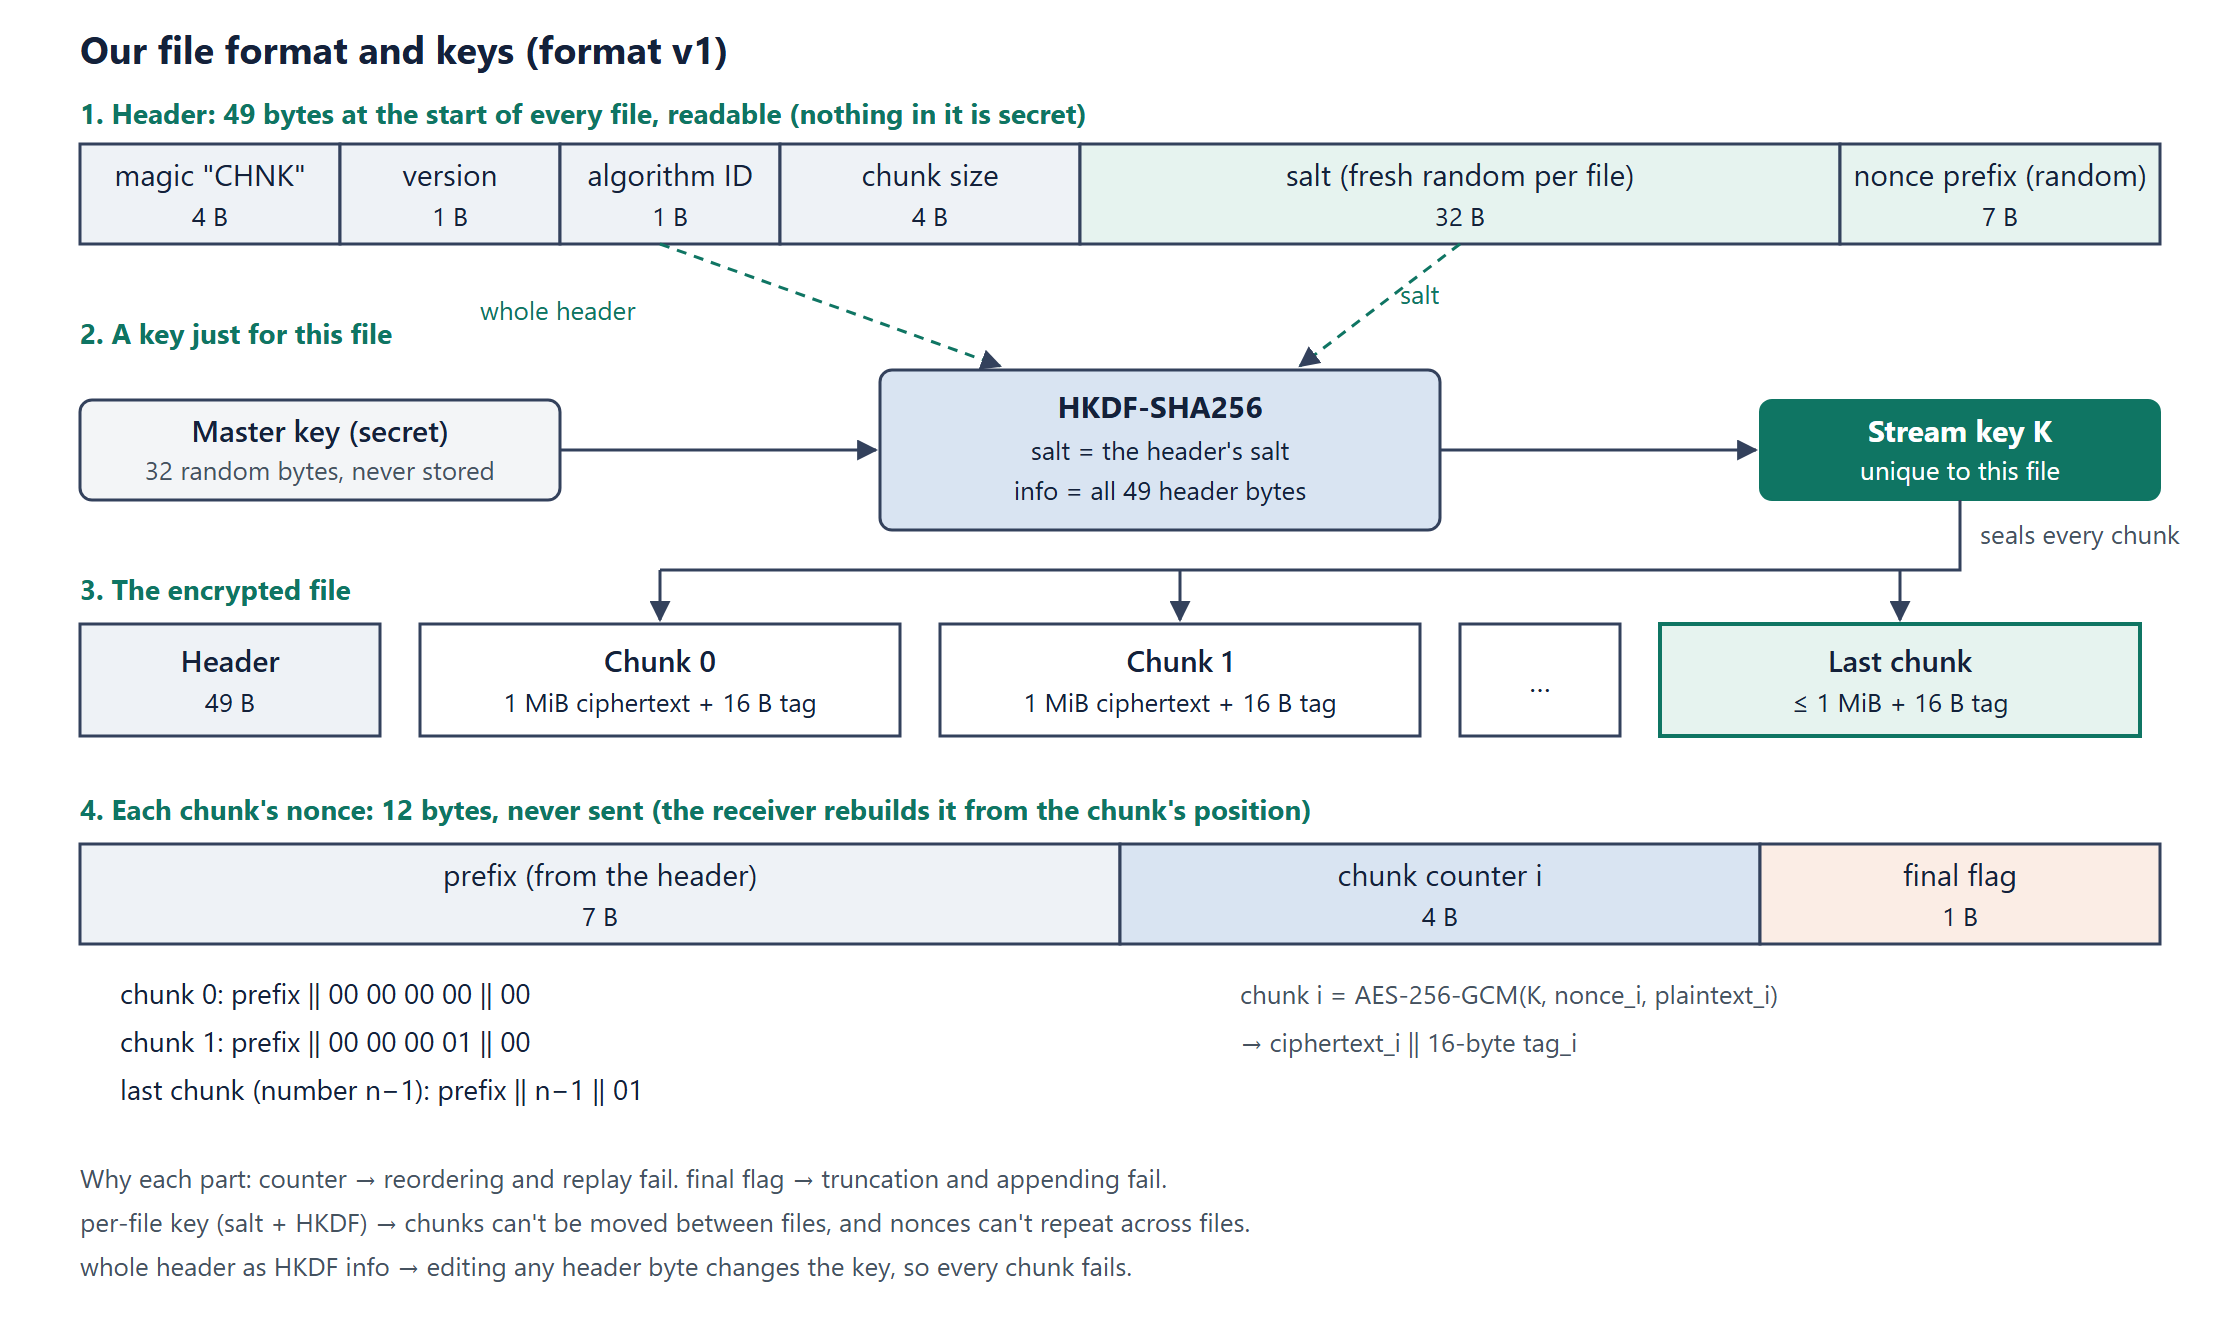
\includegraphics[width=\textwidth]{stream_format.png}
\caption{The file format: 49-byte header, per-file key, chunks, and each chunk's nonce. (The slides label the key-derivation step ``hash''; it is HKDF-SHA256.)}
\label{fig:format}
\end{figure}

Every file starts with a 49-byte header in the clear (Figure~\ref{fig:format}); nothing in it is secret.

\begin{center}
\begin{tabularx}{\textwidth}{llX}
\toprule
Field & Size & Purpose\\
\midrule
Magic \texttt{"CHNK"} & 4\,B & Reject files that are not ours immediately.\\
Version & 1\,B & Lets the format change without misreading old files.\\
Algorithm ID & 1\,B & Names the cipher, so a later version can add another.\\
Chunk size & 4\,B & Tells the decryptor where chunks end; capped at 16\,MiB so a forged header cannot force a huge read.\\
Salt & 32\,B & Random per file; makes the file key unique.\\
Nonce prefix & 7\,B & Random per file; the first 7 bytes of every nonce.\\
\bottomrule
\end{tabularx}
\end{center}

\subsection{Per-file key}
\[
K_{\mathrm{file}} = \mathrm{HKDF\text{-}SHA256}(K_{\mathrm{master}},\ \mathit{salt},\ \mathit{info} = \text{all 49 header bytes}).
\]
A key per file means a chunk from another file fails to verify (splicing), files cannot share a (key, IV) pair unless their salts collide, and learning one file's key does not reveal the master key or any other file. Because the whole header is the \emph{info} label, changing any header byte changes the key and every chunk fails, so the header is authenticated without being encrypted.

\subsection{Nonce}
Chunk $i$ uses the 96-bit nonce $N_i = \mathit{prefix} \cat \mathrm{BE}_{32}(i) \cat f_i$, where $f_i = 1$ only for the last chunk. The counter binds each chunk to its position, defeating reordering and replay, and makes nonces within a file unique; encryption stops rather than wrap at $2^{32}$ chunks, which at 1\,MiB per chunk allows 4\,PiB. The final flag defeats truncation and appended data. The nonce is never stored: the decryptor rebuilds it from the chunk's position, so a moved chunk cannot be repaired by editing a nonce.

\subsection{Streaming engine}

\begin{figure}[ht]
\centering
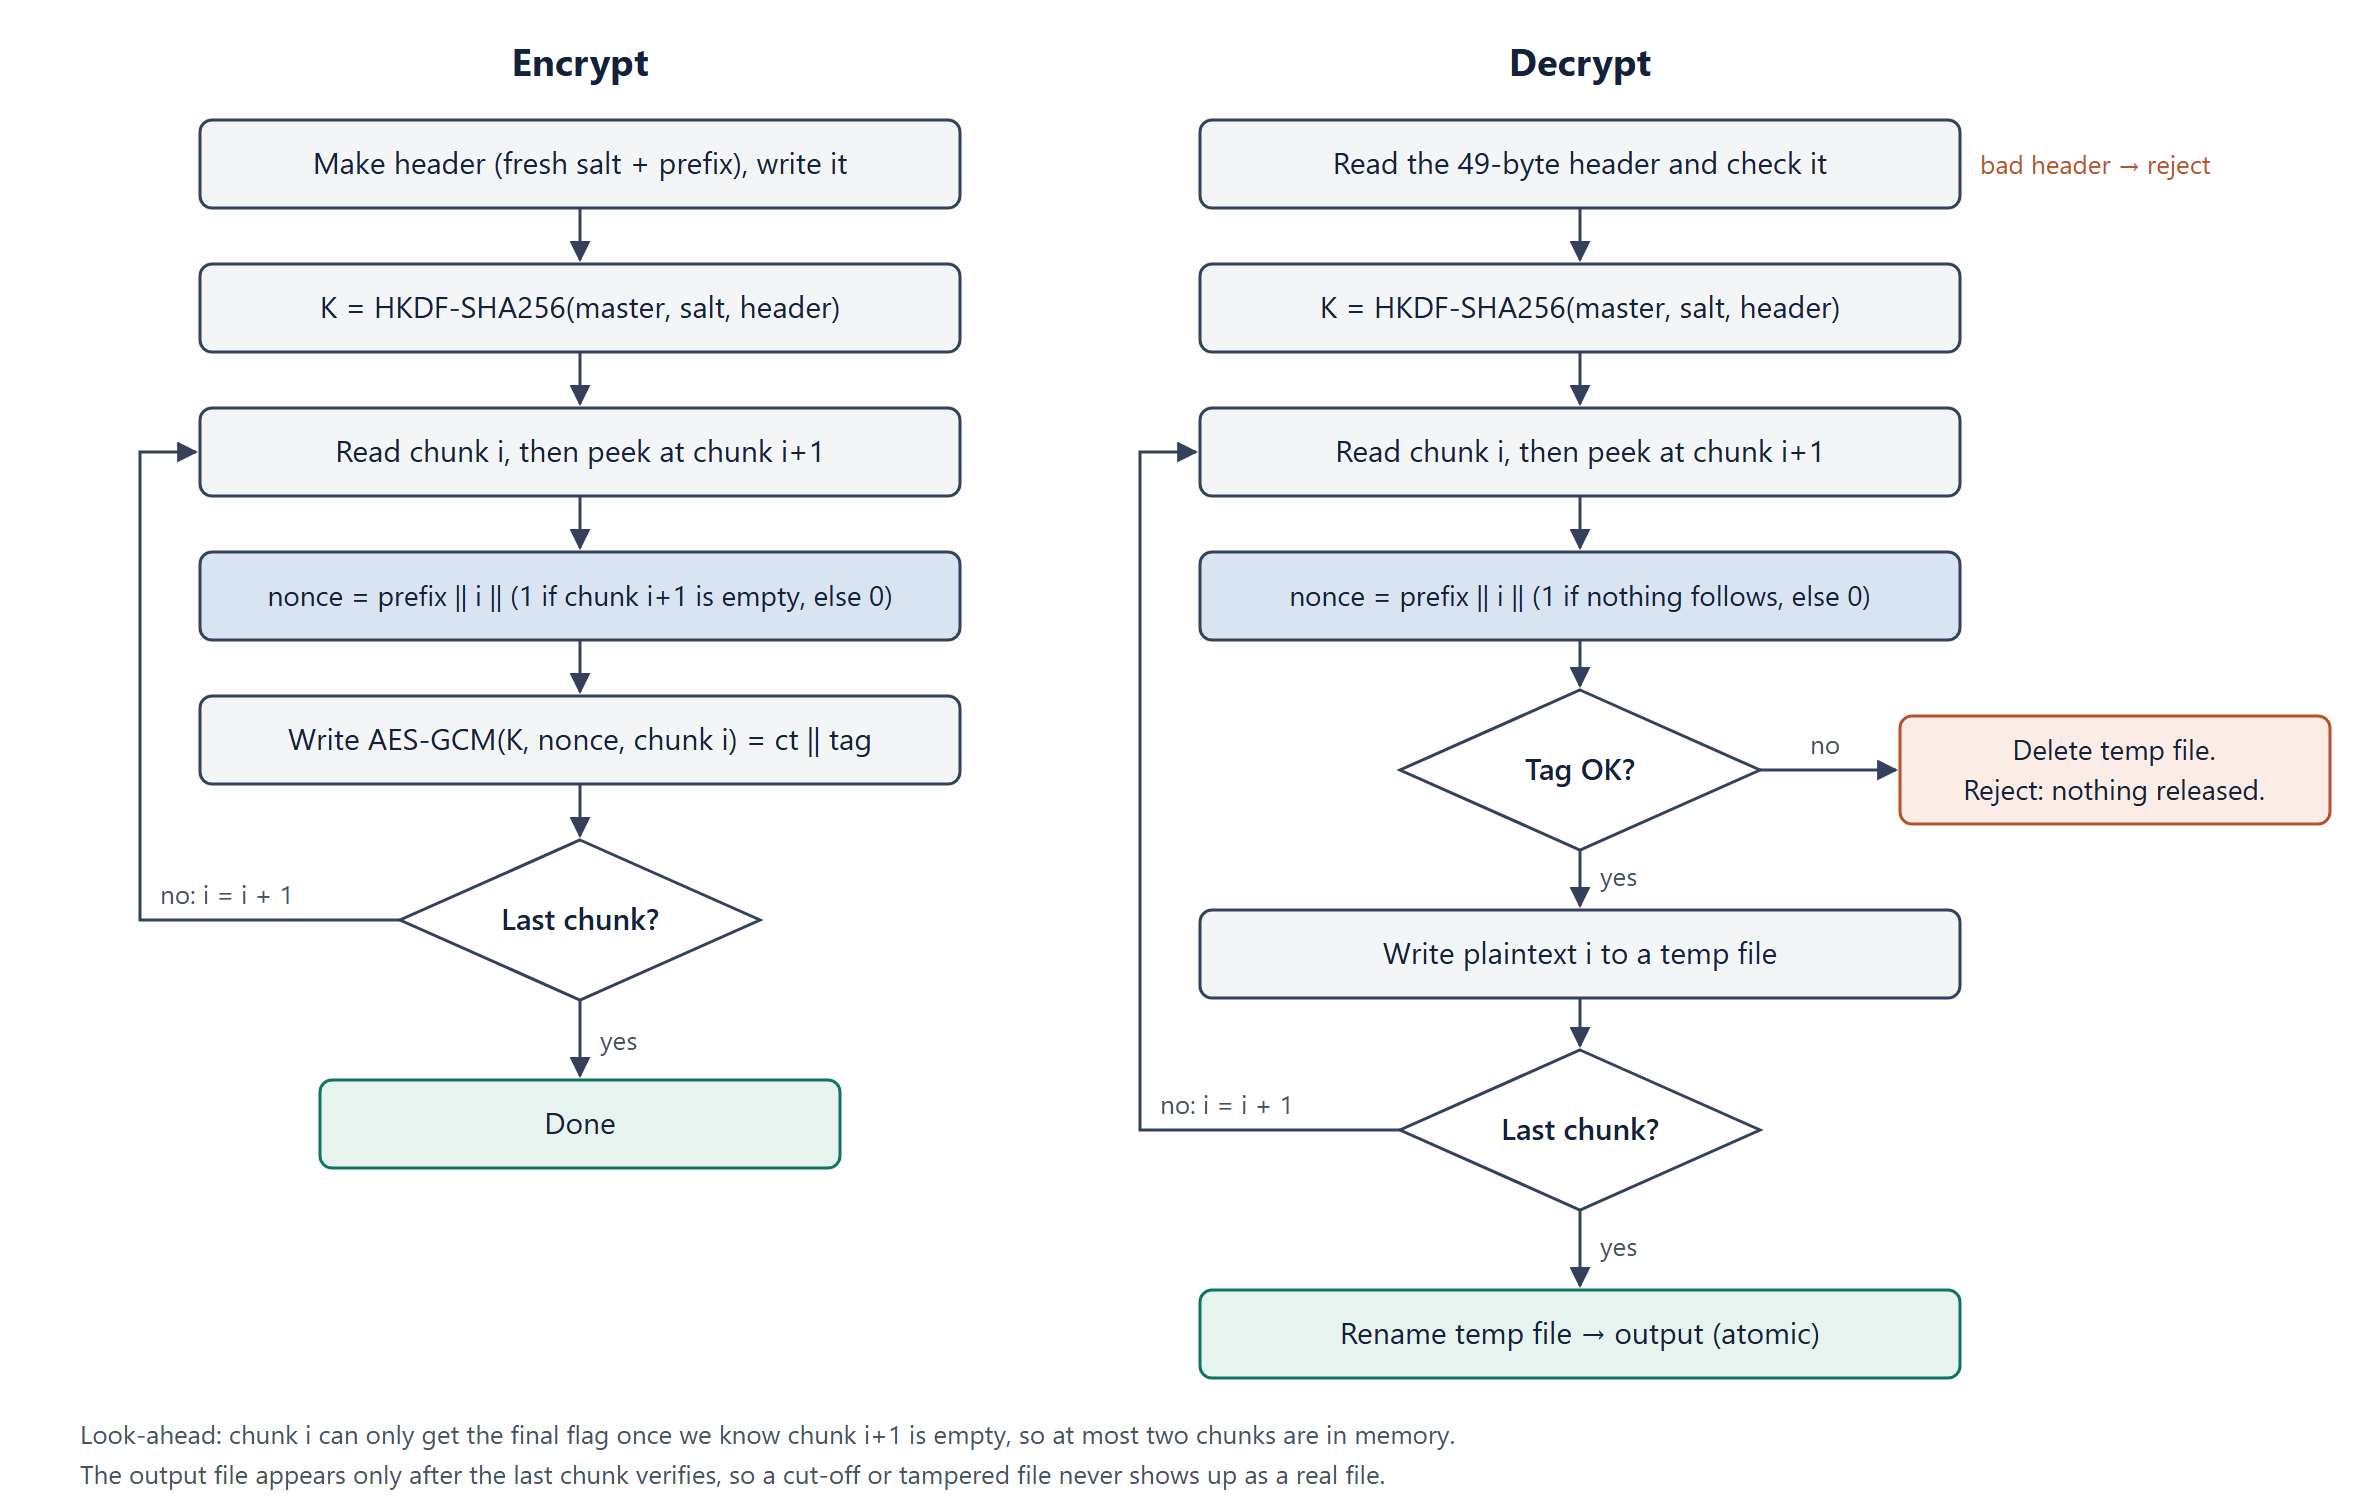
\includegraphics[width=0.95\textwidth]{stream_flow.png}
\caption{Encryption and decryption: look-ahead by one chunk, verify before writing, rename into place at the end.}
\label{fig:flow}
\end{figure}

The encryptor reads chunk $i+1$ before sealing chunk $i$, since a chunk can only receive the final flag once nothing follows it (Figure~\ref{fig:flow}); at most two chunks are in memory. An empty file still yields one empty final chunk. The encryptor generates its own salt and prefix and refuses to run twice, so a retry can never repeat an IV. The decryptor checks each chunk's tag before writing its plaintext to a temporary file, which is renamed into place (\texttt{os.replace}, atomic) only after the last chunk verifies and deleted on any failure. Reads repeat until a chunk is full, so the engine also works over sockets and pipes.

\subsection{Naive baseline and attack suite}
For comparison we implemented a naive design: the file is divided into chunks and each is encrypted with independent AES-GCM under the master key, with a random 12-byte IV stored before the chunk. It has no per-file key, its IVs say nothing about position, and nothing marks the end. A script runs five attacks against both designs: truncation (drop the last chunk), reordering (swap chunks 0 and 1), replay (repeat chunk 1), splicing (insert a chunk from another file encrypted under the same master key) and IV reuse (two messages under the same key and IV).

\subsection{Experimental setup}
All measurements were taken on an AMD Ryzen 7 7745HX laptop with 15\,GB RAM, Windows 11, Python 3.12 and \texttt{cryptography} 50. Correctness is checked with 94 automated tests (\texttt{pytest}) and NIST's test files. Peak memory is measured with \texttt{tracemalloc}, which counts the memory Python code allocates, and time with \texttt{time.perf\_counter()}. Throughput runs discard the output, so disk speed is not measured.

%=====================================================================
\section{Experimental results and analysis}

\subsection{Conformance of our GCM}
Our GCM passes all 47,250 records of NIST's six GCM test files (encryption and decryption, 128-, 192- and 256-bit keys, tags of 32 to 128 bits, IVs of several lengths), including rejecting every record marked as a failure. On random inputs its output is byte-for-byte identical to OpenSSL's, and a stream encrypted with one implementation decrypts with the other. Corrupting a single table entry makes 1,368 vectors in one file fail, which confirms the tests detect errors.

\subsection{Attacks 1--4: moving valid chunks}
\begin{center}
\begin{tabular}{llll}
\toprule
Attack & Naive & Ours & What stops it in ours\\
\midrule
Truncation & accepted & rejected & Final flag in the nonce\\
Reordering & accepted & rejected & Counter in the nonce\\
Replay & accepted & rejected & Counter in the nonce\\
Splicing & accepted & rejected & Per-file key (salt + HKDF)\\
\bottomrule
\end{tabular}
\end{center}
In every case each chunk still passes its own GCM tag check: these attacks never break GCM, they only move valid chunks. The naive decryptor therefore outputs a shortened, reordered, duplicated or mixed file without any error. Ours rejects each one, because the decryptor expects a specific nonce at each position, under a key specific to the file, and a moved or missing chunk was sealed with a different one.

\subsection{Attack 5: IV reuse under the same key}
Suppose two messages $(A_1, X_1)$ and $(A_2, X_2)$ are encrypted under the same key and IV, giving $(A_1, Y_1, t_1)$ and $(A_2, Y_2, t_2)$, and the attacker knows $X_1$.

\paragraph{Confidentiality fails.} The keystream is $S = X_1 \oplus Y_1$, so $X_2 = Y_2 \oplus S$ for as many bits as both messages share.

\paragraph{Authentication fails (the forbidden attack).} Both tags share the same mask $E_K(J_0)$:
\[ t_j = \mathrm{GHASH}_H(A_j, Y_j) \oplus E_K(J_0), \qquad j = 1, 2. \]
Adding them gives
\[
t_1 \oplus t_2 \oplus \mathrm{GHASH}_H(A_1, Y_1) \oplus \mathrm{GHASH}_H(A_2, Y_2) = 0,
\]
a polynomial in $H$ whose roots are candidates for $H$. Then $E_K(J_0) = t_1 \oplus \mathrm{GHASH}_H(A_1, Y_1)$, and for any chosen message the attacker computes $Y' = X' \oplus S$ and a valid tag $t' = \mathrm{GHASH}_H(A', Y') \oplus E_K(J_0)$.

For two one-block messages without associated data the polynomial reduces to $t_1 \oplus t_2 = (Y_1 \oplus Y_2) H^2$, so $H = \big((t_1\oplus t_2)/(Y_1\oplus Y_2)\big)^{2^{127}}$, the unique square root. Our attack script recovers the true $H$ this way, and the naive decryptor accepts a forged message (``PAY EVE 99999.99'') built with it. Against our design we force two files to share a nonce prefix: their salts, and so their keys, differ, the computed value is not $H$, and the forgery is rejected.

\subsection{Why IV reuse can only be made improbable}
IV reuse is a limitation of GCM itself, so no design built on GCM can survive it; ours prevents it instead.
\begin{itemize}
\item \textbf{Within a file:} every nonce contains the chunk counter, which never repeats and never wraps, so the probability of a repeat is zero.
\item \textbf{Between two files:} a shared key and nonce requires both the 32-byte salt and the 7-byte prefix to coincide. For random values this has probability $2^{-256}\cdot 2^{-56} = 2^{-312} \approx 1.2\times 10^{-94}$ per pair of files.
\item \textbf{The naive design:} every chunk draws a random 96-bit IV under the same key, so a given pair of chunks repeats with probability $2^{-96} \approx 1.3\times 10^{-29}$, and over $q$ chunks across all files with probability about $q^2/2^{97}$, which keeps growing as more data is encrypted.
\item \textbf{If a key leaks:} in the naive design the master key encrypts every file, so all files are exposed. In ours a leaked file key exposes that file only; HKDF does not reveal the master key.
\end{itemize}

\subsection{Throughput and chunk size}
\begin{center}
\begin{tabular}{lrrrr}
\toprule
Chunk size & Chunks & Median MiB/s & Range MiB/s & Size overhead\\
\midrule
4 KiB & 32,768 & 1,506 & 1,472--1,531 & 0.3907\%\\
16 KiB & 8,192 & 3,807 & 3,587--3,872 & 0.0977\%\\
64 KiB & 2,048 & 6,468 & 6,133--6,625 & 0.0245\%\\
256 KiB & 512 & 7,966 & 7,474--8,104 & 0.0061\%\\
\textbf{1 MiB} & \textbf{128} & \textbf{2,498} & \textbf{2,441--2,538} & \textbf{0.0016\%}\\
4 MiB & 32 & 3,037 & 2,962--3,071 & 0.0004\%\\
16 MiB & 8 & 3,043 & 2,883--3,145 & 0.0001\%\\
one-shot AES-GCM & 1 & 5,533 & & 0.000012\%\\
\bottomrule
\end{tabular}
\end{center}
Throughput for encrypting 128\,MiB, median of five interleaved rounds. Very small chunks are slow because the fixed cost per chunk dominates. Every size from 16\,KiB up exceeds the speed of a typical SSD, so throughput does not decide the chunk size. 64\,KiB is fastest but limits a file to $2^{32}\times 64$\,KiB $=256$\,TiB; 256\,KiB was fast in this run but measured 2,170--5,170\,MiB/s in another, as it sits at the edge of the CPU cache. 1\,MiB is stable, has 0.0016\% overhead and allows 4\,PiB, so it is our default; the chunk size is stored in the header, so other sizes remain readable.

\subsection{Memory and time}
\begin{center}
\begin{tabular}{lr}
\toprule
Measurement & Result\\
\midrule
Peak memory, our engine, 256\,MiB file, 1\,MiB chunks & 3.01\,MiB\\
Peak memory, one-shot AES-GCM, same file & 512.01\,MiB\\
Peak memory, our engine, 5\,MiB and 50\,MiB files (encrypt and decrypt) & 3.02\,MiB each\\
Sealing one 1\,MiB chunk, our pure-Python GCM & 162\,ms\\
Sealing one 1\,MiB chunk, OpenSSL (AES-NI, PCLMULQDQ) & 0.23\,ms\\
\bottomrule
\end{tabular}
\end{center}
Our engine's memory does not grow with the file: the peak is three 1\,MiB buffers (the current chunk, the look-ahead chunk and the output), against the whole input plus the whole output for one-shot GCM. Our GCM is about 700 times slower than OpenSSL, which uses dedicated CPU instructions for AES and for carry-less multiplication; we use it to validate and explain GCM, and OpenSSL for real encryption.

\subsection{Security of the chunked design}
Each chunk is an ordinary GCM message under a unique (key, IV) pair, so GCM's bounds apply~\cite{mv-sec}. For a 50\,GiB file ($\sigma \approx 2^{31.64}$ blocks), the confidentiality bound $(\sigma+2q)^2/2^{129}$ is $2^{-65.7}$ both as one message and as 51,200 chunks. A forgery attempt on one chunk succeeds with probability about $2^{16}/2^{128} = 2^{-112}$; one attempt on every chunk totals $2^{-96.4}$, the same as one attempt on the whole message. Chunking therefore keeps GCM's security bounds, provided IVs never repeat and each file has its own key.

%=====================================================================
\section{Conclusions}
We implemented AES-GCM from its definition, validated it against all 47,250 NIST test vectors, and built a chunked file format over it that encrypts files of any size in about 3\,MiB of memory. Per-file keys and nonces that encode each chunk's position and whether it is last stop truncation, reordering, replay and splicing, all of which succeed against a naive chunked design. IV reuse breaks GCM itself, so it cannot be survived, only prevented; our design makes it impossible within a file and negligible between files ($2^{-312}$ per pair), where the naive design's risk grows with every chunk encrypted.

\paragraph{Limitations and future work.} An attacker can replace a file with an older genuine version, which needs version numbers at a higher layer to detect. The design relies on the system's random number generator. Our Python GCM is not constant-time and is used only for validation. Natural extensions are password-based keys (Argon2 before HKDF), a second algorithm for processors without AES instructions, and random access to individual chunks, which the positional nonces allow.

\paragraph{Use of AI assistance.} We used an LLM to help write code and documentation. Every result above is reproduced by the repository's tests and scripts.

%=====================================================================
\section{References}
\begingroup
\renewcommand{\section}[2]{}
\begin{thebibliography}{99}
\bibitem{mv-spec} D.~A.~McGrew and J.~Viega, \emph{The Galois/Counter Mode of Operation (GCM)}, submission to NIST, 2005.
\bibitem{mv-sec} D.~A.~McGrew and J.~Viega, \emph{The Security and Performance of the Galois/Counter Mode (GCM) of Operation}, INDOCRYPT 2004; IACR ePrint 2004/193.
\bibitem{sp80038d} M.~Dworkin, \emph{Recommendation for Block Cipher Modes of Operation: Galois/Counter Mode (GCM) and GMAC}, NIST SP 800-38D, 2007.
\bibitem{fips197} NIST, \emph{Advanced Encryption Standard (AES)}, FIPS 197, 2001.
\bibitem{cavp} NIST Cryptographic Algorithm Validation Program, \emph{GCM Validation System (GCMVS) test vectors}, CAVS 14.0.
\bibitem{rfc5869} H.~Krawczyk and P.~Eronen, \emph{HMAC-based Extract-and-Expand Key Derivation Function (HKDF)}, RFC 5869, 2010.
\bibitem{hrrv} V.~T.~Hoang, R.~Reyhanitabar, P.~Rogaway and D.~Viz\'ar, \emph{Online Authenticated-Encryption and its Nonce-Reuse Misuse-Resistance}, CRYPTO 2015.
\bibitem{iom} T.~Iwata, K.~Ohashi and K.~Minematsu, \emph{Breaking and Repairing GCM Security Proofs}, CRYPTO 2012.
\bibitem{joux} A.~Joux, \emph{Authentication Failures in NIST Version of GCM}, comment to NIST, 2006.
\bibitem{shoup} V.~Shoup, \emph{On Fast and Provably Secure Message Authentication Based on Universal Hashing}, CRYPTO 1996.
\bibitem{tink} Google, \emph{Tink: Streaming AEAD (AES-GCM-HKDF)}, \url{https://developers.google.com/tink}.
\bibitem{age} F.~Valsorda and B.~Cartwright-Cox, \emph{The age file encryption format}, \url{https://c2sp.org/age}.
\bibitem{rfc8446} E.~Rescorla, \emph{The Transport Layer Security (TLS) Protocol Version 1.3}, RFC 8446, 2018.
\end{thebibliography}
\endgroup

\end{document}
